\documentclass[10pt,a4paper]{article}

\usepackage[utf8]{inputenc}
\usepackage[T1]{fontenc}
\usepackage{amsmath,amssymb,amsfonts}
\usepackage{graphicx}
\usepackage{hyperref}
\usepackage{algorithm}
\usepackage{algpseudocode}
\usepackage{multicol}
\usepackage{geometry}
\usepackage{cite}
\usepackage{authblk}

% Mise en page
\geometry{margin=2cm}

% Page de titre
\title{\Large\textbf{TPTT : Transformation de Transformers Pré-entraînés en Titans}}
\author{\large Fabien Furfaro\thanks{\texttt{fabien.furfaro@gmail.com}}}
\date{\large 2025}

\begin{document}

\maketitle

\begin{abstract}
Les avancées récentes dans les grands modèles de langage (LLMs) ont permis des progrès remarquables en traitement automatique du langage naturel, mais leurs demandes computationnelles et mémorielles restent un défi majeur, en particulier pour l'inférence en contexte long. Nous présentons TPTT (Transforming Pretrained Transformer into Titans), un nouveau cadre pour améliorer les modèles Transformer pré-entraînés avec des mécanismes d'attention linéarisés efficaces et une gestion avancée de la mémoire. TPTT tire parti de techniques telles que la Mémoire comme Porte (MaG) et l'attention linéarisée mixte (LiZA), et est entièrement compatible avec la bibliothèque Hugging Face Transformers, permettant une adaptation transparente de tout LLM causal via un ajustement fin paramétrique efficace (LoRA) sans réentraînement complet. Nous démontrons l'efficacité de TPTT sur le benchmark MMLU avec des modèles d'environ 1 milliard de paramètres, observant des améliorations substantielles en termes d'efficacité et de précision. Par exemple, Titans-Llama-3.2-1B atteint une augmentation de 20\% en Exact Match (EM) par rapport à sa référence. Des analyses statistiques détaillées et des comparaisons avec les méthodes récentes de l'état de l'art confirment la scalabilité pratique et la robustesse de TPTT. Le code source est disponible à l'adresse \url{https://github.com/fabienfrfr/tptt}.
\end{abstract}

\begin{figure}[ht]
    \centering
    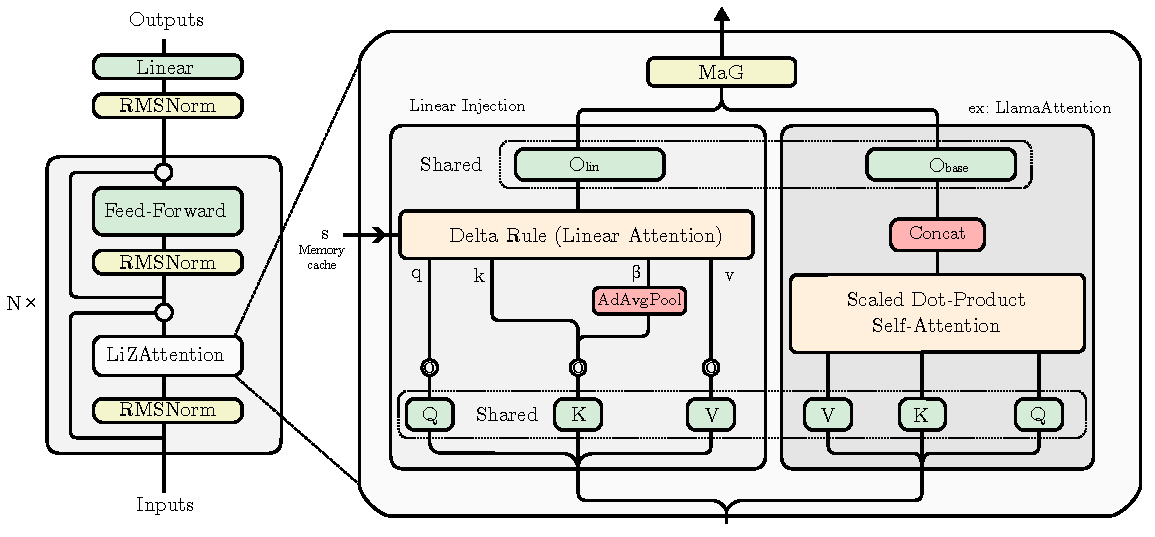
\includegraphics[width=0.8\linewidth]{fig.pdf}
    \caption{Aperçu de l'architecture du cadre TPTT. À gauche, le diagramme illustre une architecture de décodeur où l'attention linéaire est injectée en parallèle de l'attention vanille (LiZAttention). À droite, l'architecture détaillée du mécanisme d'attention linéarisée est représentée, mettant en évidence les poids partagés pour les projections de requête (Q), de clé (K) et de valeur (V). Il montre également la gestion de la mémoire d'état (S) et la combinaison des sorties par le mécanisme de pondération Memory as Gate (MaG). Le diagramme met l'accent sur l'intégration des mécanismes d'attention linéarisée et des techniques avancées de gestion de la mémoire, telles que Delta Rule et AdaptativeAvgPool1D, contribuant au traitement et à la génération de sorties.}
    \label{fig:approach_overview}
\end{figure}

\section{Introduction}

Le succès des grands modèles de langage basés sur les transformeurs (LLMs)~\cite{vaswani2017attention, mann2020language} a révolutionné le traitement automatique du langage naturel (NLP), permettant des progrès sans précédent dans une large gamme de tâches. Cependant, la complexité computationnelle quadratique et les exigences substantielles en mémoire du mécanisme d'auto-attention standard restent un goulot d'étranglement significatif, en particulier pour l'inférence en contexte long.

Pour relever ces défis, des recherches récentes ont exploré plusieurs directions. Des mécanismes d'attention efficaces~\cite{katharopoulos2020transformers, yang2024parallelizing} ont été proposés pour réduire la complexité de l'auto-attention de quadratique à linéaire ou quasi-linéaire, la rendant plus tractable pour les longues séquences. Des architectures récurrentes et des mécanismes de mémoire interne~\cite{mercat2024linearizing, behrouz2024titans} ont également été développés pour améliorer la capacité du modèle à capturer les dépendances à long terme, s'inspirant de la mémoire cognitive dans les systèmes biologiques plutôt que de la mémoire matérielle. De plus, des approches d'ajustement fin paramétrique efficaces telles que LoRA~\cite{hu2022lora} permettent l'adaptation de grands modèles pré-entraînés à de nouvelles tâches sans avoir besoin d'un réentraînement complet.

\section{Travaux Connexes}

Malgré ces avancées, la plupart des méthodes existantes nécessitent des modifications architecturales significatives ou un entraînement à partir de zéro, ce qui limite leur applicabilité aux modèles déjà pré-entraînés. Par exemple, des solutions comme FlashAttention~\cite{dao2023flashattention} et Mamba~\cite{gu2023mamba} se concentrent sur des architectures efficaces, tandis que d'autres comme LoLCat~\cite{zhang2024lolcats} et Liger~\cite{lan2025liger} convertissent l'attention standard en formes linéarisées ; notamment, Liger exploite des propriétés similaires à celles utilisées dans ce travail, mais ne repose pas sur une injection de linéarisation explicite.

Dans ce travail, nous introduisons TPTT (Transforming Pretrained Transformer into Titans), un cadre qui transforme les modèles de transformateurs pré-entraînés en architectures plus efficaces et scalables en incorporant des mécanismes d'attention linéarisés et une augmentation avancée de la mémoire interne. TPTT tire parti de techniques telles que la Mémoire comme Porte (MaG) et l'attention linéarisée mixte (LiZA), s'inspirant de l'architecture Titans~\cite{behrouz2024titans}. Notre approche est entièrement compatible avec les cadres existants et permet une adaptation rapide de tout LLM causal à des tâches à long contexte via un ajustement fin paramétrique efficace avec LoRA~\cite{hu2022lora}, sans nécessiter de réentraînement complet. L'objectif est de débloquer le potentiel des modèles déjà entraînés en les équipant de capacités augmentées par la mémoire grâce à une adaptation légère.

\section{Methodologie}

\subsection{Mécanismes d'Attention Linéarisés}

L'auto-attention standard dans les transformeurs calcule les interactions par paires entre tous les jetons, ce qui entraîne une complexité quadratique par rapport à la longueur de la séquence~\cite{vaswani2017attention}. Pour remédier à cela, les mécanismes d'attention linéarisés approximient l'attention softmax en utilisant des opérations linéaires, généralement en projetant les requêtes et les clés à travers une carte de caractéristiques $\phi$~\cite{katharopoulos2020transformers, wang2020linformer, mercat2024linearizing, yang2024parallelizing}. Cela réduit les coûts computationnels et mémoriels, permettant un traitement efficace des longues séquences tout en maintenant la puissance de modélisation~\cite{gu2023mamba, dao2023flashattention, zhang2024lolcats, lan2025liger}. La sortie de l'attention softmax pour une séquence d'entrée $\mathbf{X} = \{\mathbf{x}_1, \dots, \mathbf{x}_T\} \in \mathbb{R}^{T \times D}$ est :
\begin{equation}
\mathbf{Q}, \mathbf{K}, \mathbf{V} = \mathbf{X}\mathbf{W}_Q, \mathbf{X}\mathbf{W}_K, \mathbf{X}\mathbf{W}_V
\end{equation}
\begin{equation}
\mathbf{O}_{\text{base}} = \text{Softmax}\left(\frac{\mathbf{Q}\mathbf{K}^\top}{\sqrt{D}}\right)\mathbf{V}
\end{equation}
En attention linéaire, cela est approximé comme suit :
\begin{equation}
\mathbf{O}_{\text{lin}, (t)} = \frac{\sum_{i=1}^{t} \phi(\mathbf{q}_t)^\top \phi(\mathbf{k}_i) \mathbf{v}_i}{\sum_{i=1}^{t} \phi(\mathbf{q}_t)^\top \phi(\mathbf{k}_i)}
\end{equation}
où $\phi$ est une fonction de mappage de caractéristiques, telle que ELU ou des approximations de noyau~\cite{wang2020linformer}.

\subsection{Mémoire comme Porte (MaG)}

Pour améliorer davantage la modélisation des dépendances à long terme, nous introduisons un mécanisme d'augmentation de la mémoire interne, Mémoire comme Porte (MaG), inspiré de l'architecture Titans~\cite{behrouz2024titans}. Contrairement à la mémoire matérielle, ce mécanisme permet au modèle de stocker et de rappeler des informations contextuelles sur des séquences étendues, de manière analogue à la mémoire cognitive. MaG combine les sorties de l'attention standard et linéarisée en utilisant un paramètre de pondération :
\begin{equation}
\mathbf{O} = \alpha \cdot \mathbf{O}_{\text{lin}} + (1-\alpha) \cdot \mathbf{O}_{\text{base}}
\end{equation}
où $\alpha \in [0,1]$ est adapté pendant l'entraînement. Cela permet au modèle de tirer parti à la fois de l'efficacité de l'attention linéaire et de l'expressivité de l'attention softmax, et peut être vu comme une forme de gating augmentée par la mémoire~\cite{behrouz2024titans, mercat2024linearizing}.

\subsection{Modélisation Parallèle de la Règle Delta}

Dans ce travail, la fonction de mappage des caractéristiques de l'attention linéaire est approximée par DeltaNet~\cite{yang2024parallelizing}. La mise à jour récurrente des états de mémoire interne est formulée de deux manières, suivant :
\begin{itemize}
    \item \textbf{Forme Fermée (intra-chunk) :}
    \begin{equation}
    \mathbf{S}_t = \mathbf{S}_{t-1} + \sum_{i=1}^{C} \mathbf{v}_i \mathbf{k}_i^\top
    \end{equation}
    où $C$ est la taille du chunk et $\mathbf{S}_t$ est l'état mis à jour.
    \item \textbf{Forme Récurrente (inter-chunk) :}
    \begin{equation}
    \mathbf{S}_{t+1} = \mathbf{S}_t + \mathbf{v}_{t+1} \mathbf{k}_{t+1}^\top
    \end{equation}
    L'état final d'un chunk devient l'état initial du suivant, soutenant une utilisation efficace de la mémoire pour les longues séquences.
\end{itemize}
La sortie $\mathbf{O}_{\text{lin}}$ est ensuite calculée à partir de ces états de mémoire.

\subsection{Intégration avec les Modèles Pré-entraînés}

Notre approche injecte des modules d'attention linéarisés et d'augmentation de mémoire dans les modèles de transformateurs pré-entraînés. Le processus implique :
\begin{enumerate}
    \item \textbf{Identification des Modules Cibles :} Les couches d'attention clés à modifier sont identifiées à l'aide d'outils tels que \texttt{get\_tptt\_model}.
    \item \textbf{Modification des Couches d'Attention :} Ces couches sont remplacées ou étendues avec le module proposé \texttt{LiZAttention}, qui implémente à la fois l'attention linéaire et softmax avec un partage de poids de projection linéaire et MaG.
    \item \textbf{Entraînement et Ajustement Fin :} Le modèle modifié est ajusté finement en utilisant des méthodes paramétriques efficaces telles que LoRA~\cite{hu2022lora}, assurant une adaptation optimale aux nouveaux mécanismes sans réentraînement complet.
\end{enumerate}
Cette procédure permet la transformation de tout LLM causal pré-entraîné en une architecture efficace augmentée de mémoire avec un minimum de surcharge, et ce sans aucune nouvelle couche.

\subsection{Module LiZAttention}

Le module \texttt{LiZAttention} est un composant central de l'architecture TPTT, conçu pour combiner de manière synergique les mécanismes d'attention linéarisée et standard (softmax). Cette approche hybride tire parti de l'efficacité computationnelle de l'attention linéaire tout en conservant l'expressivité de l'attention vanille. Pour soutenir l'inférence en contexte long, \texttt{LiZAttention} maintient un cache d'états intermédiaires et implémente un mécanisme d'information récurrente pour une gestion efficace de la mémoire interne~\cite{katharopoulos2020transformers}.

\begin{algorithm}[H]
\caption{Passe Avant de LiZAttention}
\label{alg:lizattention}
\begin{algorithmic}[1]
\Require $\text{hidden\_states} \in \mathbb{R}^{B \times L \times D}$ \Comment{Taille du lot $B$, longueur de la séquence $L$, dimension d'intégration $D$}
\Require $\text{mask}$ \Comment{Masque d'attention pour le padding/la causalité}
\State \textbf{Projection :}
    \Statex \hspace{1em} Calculer les requêtes $q$, les clés $k$, les valeurs $v$ via des projections apprises :
    \Statex \hspace{1em} $q \in \mathbb{R}^{B \times H \times L \times d_h}$, $k, v \in \mathbb{R}^{B \times H_k \times L \times d_h}$
\State \textbf{Appliquer le Masque d'Attention :}
    \Statex \hspace{1em} Appliquer $\text{mask}$ à $k$ et $v$ pour gérer le padding et restreindre l'attention.
\State \textbf{Attention Linéaire :}
    \Statex \hspace{1em} Calculer la sortie de l'attention linéaire $o_{\mathrm{lin}}$ en utilisant une carte de caractéristiques $\phi$ :
    \Statex \hspace{1em} $o_{\mathrm{lin}}[t] = \frac{\sum_{i=1}^{t} \phi(q_t)^\top \phi(k_i) v_i}{\sum_{i=1}^{t} \phi(q_t)^\top \phi(k_i)}$
    \Statex \hspace{1em} Stocker les états intermédiaires dans un cache mémoire pour l'information récurrente.
\State \textbf{Attention Vanille (Softmax) :}
    \Statex \hspace{1em} Calculer la sortie de l'auto-attention standard $o_{\mathrm{base}}$ (optionnellement tronquée pour les longues séquences) :
    \Statex \hspace{1em} $o_{\mathrm{base}} = \text{Softmax}\left(\frac{q k^\top}{\sqrt{d_h}}\right) v$
\State \textbf{Combiner les Sorties (Mémoire comme Porte) :}
    \Statex \hspace{1em} Calculer la sortie finale en utilisant un paramètre de porte apprise $\alpha$ :
    \Statex \hspace{1em} $o = \alpha \cdot o_{\mathrm{lin}} + (1-\alpha) \cdot o_{\mathrm{base}}$
\State \Return $o \in \mathbb{R}^{B \times L \times D}$
\end{algorithmic}
\end{algorithm}

\subsubsection{Gestion Efficace de la Mémoire Interne}

Le cache d'états intermédiaires maintenu par \texttt{LiZAttention} permet une information récurrente, soutenant efficacement l'inférence en contexte long sans surcharge computationnelle excessive~\cite{katharopoulos2020transformers}. Cette approche permet au modèle de passer à l'échelle pour des séquences plus longues, en tirant parti à la fois du contexte local et global.

\section{Procédure d'Entraînement}

\subsection{Ajustement Fin Efficace des Paramètres avec LoRA}

Pour adapter l'architecture TPTT aux tâches en aval, nous employons l'Adaptation de Faible Rang (LoRA)~\cite{hu2022lora, lora_hf}, une technique d'ajustement fin efficace des paramètres qui injecte des matrices de faible rang entraînables dans des couches de projection sélectionnées tout en gelant les poids du modèle d'origine. Cette approche réduit considérablement le nombre de paramètres entraînables et les exigences en mémoire, tout en maintenant des performances comparables à un ajustement fin complet~\cite{hu2022lora, lora_hf}. Pour TPTT, LoRA est configuré avec un rang de 8, $\alpha=16$, et un taux de dropout de 0,05. L'ajustement fin cible les modules de projection principaux, spécifiquement \texttt{[q\_proj, k\_proj, v\_proj, o\_proj]} pour Llama/Mistral et \texttt{[qkv\_proj, out\_proj]} pour OpenELM~\cite{lora_hf}.

\subsection{Planification Dynamique de la Mémoire comme Porte (Callback LiZA MaG)}

Un composant critique du processus d'entraînement est le callback LiZA MaG, qui ajuste dynamiquement le paramètre de pondération Mémoire comme Porte (MaG) pendant l'entraînement. Le poids MaG est initialisé à 0,01 et augmenté linéairement à 0,5 sur les 100 premières étapes, facilitant une transition en douceur de la dépendance à l'attention vanille (softmax) vers l'attention linéarisée. Cet horaire permet au modèle d'équilibrer efficacement les deux mécanismes d'attention, optimisant les performances tout au long de l'entraînement. Le callback est intégré directement dans la boucle d'entraînement, assurant un contrôle adaptatif du paramètre MaG et améliorant l'adaptabilité et l'efficacité du modèle.

\section{Expériences et Résultats}

\subsection{Configuration Expérimentale}

Nous avons évalué le cadre TPTT sur plusieurs modèles de langage pré-entraînés avec environ 1 milliard de paramètres, en utilisant le benchmark MMLU~\cite{hendrycks2020measuring} comme suite d'évaluation principale. L'entraînement a été effectué sur 500 échantillons du jeu de données \texttt{yahma/alpaca-cleaned}~\cite{taori2023alpaca} pendant 5 époques, avec une longueur de séquence maximale de 384 jetons, une taille de lot de 3, et un taux d'apprentissage de $5 \times 10^{-4}$. La formation mixte de précision et le clippage des gradients à 1,0 ont été employés pour optimiser l'efficacité et la stabilité computationnelles. Toutes les expériences ont été réalisées sur des GPU NVIDIA Tesla T4 (plateforme Kaggle). Les modèles entraînés et les métriques détaillées sont publics sur le Hugging Face Model Hub\footnote{\url{https://huggingface.co/ffurfaro/}}, avec des journaux d'entraînement complets accessibles via Hugging Face TensorBoard.

\subsection{Résultats de l'Entraînement}

Le tableau~\ref{tab:training-metrics} résume les métriques de performance de l'entraînement pour divers modèles TPTT. Les résultats indiquent une apprentissage constant et efficace à travers les architectures, comme en témoignent les faibles valeurs de perte finale et les normes de gradient stables. L'utilisation de l'Adaptation de Faible Rang (LoRA) et du mécanisme Mémoire comme Porte (MaG) s'est avérée efficace pour optimiser la dynamique et la convergence de l'entraînement.

\begin{table}[h!]
    \centering
    \resizebox{\textwidth}{!}{
    \begin{tabular}{|l|c|c|c|c|c|c|l|}
    \hline
    Modèle & Perte & Temps d'Entraînement (s) & Échantillons/s & Étapes/s & FLOPs Totaux & Norme du Gradient & Références Basées Sur \\
    \hline
    Titans-Llama-3.2-1B & 1,375 & 1654,1 & 1,51 & 0,254 & 5,62e18 & 2,68 & \cite{touvron2023llama} \\
    Titans-OpenELM-1\_1B & 1,3188 & 1651,1 & 1,51 & 0,254 & 5,85e18 & 0,704 & \cite{mehta2024openelm} \\
    Titans-Qwen2.5-1.5B & 1,2568 & 1900,6 & 1,31 & 0,221 & 7,56e18 & 1,99 & \cite{bai2023qwen} \\
    Titans-OLMo-1B-hf & 1,3068 & 1585,2 & 1,58 & 0,265 & 6,20e18 & 3,12 & \cite{groeneveld2024olmo} \\
    \hline
    \end{tabular}
    }
    \caption{Métriques de performance d'entraînement pour les modèles TPTT.}
    \label{tab:training-metrics}
\end{table}

\subsection{Métriques d'Évaluation et Résultats du Benchmark}

Pour l'évaluation, nous nous concentrons sur les métriques standard dans le benchmarking LLM et QA : Exact Match (EM), Partial Exact Match (PEM), et Partial Quasi Exact Match (PQEM). Ces métriques mesurent respectivement la correction stricte, le chevauchement partiel, et la quasi-exactitude entre les sorties du modèle et les réponses de vérité terrain, fournissant une vue nuancée de la performance du modèle~\cite{hendrycks2020measuring}.

Le tableau~\ref{tab:mmlu-results} présente les résultats du benchmark MMLU dans le cadre one-shot. Les modèles TPTT, et en particulier Titans-Llama-3.2-1B, surpassent systématiquement leurs homologues de base en EM, avec des scores PEM et PQEM compétitifs. Cela démontre l'avantage de l'intégration de l'attention linéarisée et des mécanismes de mémoire interne pour des tâches complexes de compréhension du langage.

\begin{table}[h!]
    \centering
    \renewcommand{\arraystretch}{1.2}
    \begin{tabular}{|l|c|c|c|}
    \hline
    Modèle & EM $\pm$ Std & PEM $\pm$ Std & PQEM $\pm$ Std \\
    \hline
    Titans-Llama-3.2-1B & 0,2456 $\pm$ 0,1276 & 0,2649 $\pm$ 0,1340 & 0,4772 $\pm$ 0,1569 \\
    Llama-3.2-1B & 0,0070 $\pm$ 0,0058 & 0,3105 $\pm$ 0,1411 & 0,4719 $\pm$ 0,1530 \\
    \hline
    Titans-Qwen2.5-1.5B & 0,0000 $\pm$ 0,0000 & 0,5000 $\pm$ 0,1504 & 0,5825 $\pm$ 0,1442 \\
    Qwen2.5-1.5B & 0,0000 $\pm$ 0,0000 & 0,5982 $\pm$ 0,1422 & 0,6895 $\pm$ 0,1288 \\
    \hline
    Titans-OLMo-1B-hf & 0,0000 $\pm$ 0,0000 & 0,2614 $\pm$ 0,1312 & 0,4649 $\pm$ 0,1540 \\
    OLMo-1B-hf & 0,0000 $\pm$ 0,0000 & 0,2333 $\pm$ 0,1302 & 0,4246 $\pm$ 0,1533 \\
    \hline
    \end{tabular}
    \caption{Résultats du benchmark MMLU (one-shot) avec analyse statistique. Chaque paire regroupe un modèle Titans et son homologue de base.}
    \label{tab:mmlu-results}
\end{table}

\subsection{Discussion et Comparaison}

Comparé aux méthodes récentes de l'état de l'art telles que Mamba~\cite{gu2023mamba}, LoLCat~\cite{zhang2024lolcats}, et Liger~\cite{lan2025liger}, TPTT se distingue en permettant la transformation de modèles pré-entraînés existants sans réentraînement complet, tout en maintenant de solides performances de benchmark. Les améliorations observées en EM et les scores compétitifs en PEM/PQEM soulignent l'efficacité de l'attention linéarisée et de l'augmentation de mémoire de TPTT pour une adaptation efficace et robuste des LLM. Ces résultats confirment que TPTT est une solution pratique et scalable pour améliorer les LLM pré-entraînés, en particulier dans des environnements contraints en ressources.

\section{Discussion et Conclusion}

Dans cet article, nous avons introduit TPTT, un nouveau cadre pour améliorer les modèles Transformer pré-entraînés en intégrant des mécanismes d'attention linéarisés efficaces et une augmentation de la mémoire interne. Notre approche utilise l'ajustement fin paramétrique efficace (LoRA)~\cite{hu2022lora} pour permettre l'adaptation rapide des grands modèles de langage (LLMs) à des tâches en contexte long, sans avoir besoin d'un réentraînement complet. Les résultats expérimentaux sur le benchmark MMLU~\cite{hendrycks2020measuring} démontrent des améliorations significatives en termes d'efficacité et de précision, avec des analyses statistiques robustes et des comparaisons favorables aux méthodes de pointe~\cite{gu2023mamba, zhang2024lolcats, lan2025liger}.

\paragraph{Implications Pratiques.}
TPTT offre une solution scalable et pratique pour déployer des LLMs haute performance dans des environnements contraints en ressources. L'intégration de mécanismes d'attention linéarisés et d'augmentation de mémoire réduit les exigences computationnelles et mémorielles, rendant les modèles de langage avancés plus accessibles pour des applications réelles. L'utilisation de LoRA permet un ajustement fin efficace et flexible, permettant une adaptation rapide à de nouvelles tâches et domaines.

\paragraph{Limitations.}
Notre évaluation actuelle est limitée à des modèles de taille modérée (environ 1 milliard de paramètres). L'échelle de TPTT à des architectures plus grandes et à des tâches plus diversifiées peut introduire de nouveaux défis, y compris une complexité d'ajustement accrue et la nécessité d'une optimisation supplémentaire des mécanismes de mémoire. Bien que nos résultats soient prometteurs, une validation plus large sur des benchmarks supplémentaires et des scénarios réels est nécessaire pour évaluer pleinement la généralisabilité et la robustesse de l'approche.

\paragraph{Directions Futures.}
Les travaux futurs se concentreront sur l'optimisation du processus d'intégration, l'exploration de mécanismes de mémoire interne plus sophistiqués~\cite{behrouz2024titans}, et l'extension de l'évaluation à des modèles plus grands et à une gamme plus large de benchmarks. Des recherches supplémentaires étudieront les approches hybrides et l'interaction entre l'attention linéarisée, l'augmentation de mémoire et d'autres techniques axées sur l'efficacité.

En résumé, TPTT fournit un cadre pratique, scalable et efficace pour la mise à niveau des Transformers pré-entraînés, avec des résultats empiriques solides et des implications prometteuses pour l'avenir de la modélisation du langage efficace.

\bibliographystyle{plain}
\bibliography{refs}

\end{document}
